\documentclass{article}
\usepackage{physics}
\usepackage{graphicx}
\usepackage{caption}
\usepackage{amsmath}
\usepackage{bm}
\usepackage{framed}
\usepackage{authblk}
\usepackage{empheq}
\usepackage{amsfonts}
\usepackage{esint}
\usepackage[makeroom]{cancel}
\usepackage{dsfont}
\usepackage{centernot}
\usepackage{mathtools}
\usepackage{subcaption}
\usepackage{bigints}
\usepackage{amsthm}
\theoremstyle{definition}
\newtheorem{lemma}{Lemma}
\newtheorem{defn}{Definition}[section]
\newtheorem{prop}{Proposition}[section]
\newtheorem{rmk}{Remark}[section]
\newtheorem{thm}{Theorem}[section]
\newtheorem{exmp}{Example}[section]
\newtheorem{prob}{Problem}[section]
\newtheorem{sln}{Solution}[section]
\newtheorem*{prob*}{Problem}
\newtheorem{exer}{Exercise}[section]
\newtheorem*{exer*}{Exercise}
\newtheorem*{sln*}{Solution}
\usepackage{empheq}
\usepackage{tensor}
\usepackage{xcolor}
%\definecolor{colby}{rgb}{0.0, 0.0, 0.5}
\definecolor{MIT}{RGB}{163, 31, 52}
\usepackage[pdftex]{hyperref}
%\hypersetup{colorlinks,urlcolor=colby}
\hypersetup{colorlinks,linkcolor={MIT},citecolor={MIT},urlcolor={MIT}}  
\usepackage[left=1in,right=1in,top=1in,bottom=1in]{geometry}

\usepackage{newpxtext,newpxmath}
\newcommand*\widefbox[1]{\fbox{\hspace{2em}#1\hspace{2em}}}

\newcommand{\p}{\partial}
\newcommand{\R}{\mathbb{R}}
\newcommand{\C}{\mathbb{C}}
\newcommand{\lag}{\mathcal{L}}
\newcommand{\nn}{\nonumber}
\newcommand{\ham}{\mathcal{H}}
\newcommand{\M}{\mathcal{M}}
\newcommand{\I}{\mathcal{I}}
\newcommand{\K}{\mathcal{K}}
\newcommand{\F}{\mathcal{F}}
\newcommand{\w}{\omega}
\newcommand{\lam}{\lambda}
\newcommand{\al}{\alpha}
\newcommand{\be}{\beta}
\newcommand{\x}{\xi}

\newcommand{\G}{\mathcal{G}}

\newcommand{\f}[2]{\frac{#1}{#2}}

\newcommand{\ift}{\infty}

\newcommand{\lp}{\left(}
\newcommand{\rp}{\right)}

\newcommand{\lb}{\left[}
\newcommand{\rb}{\right]}

\newcommand{\lc}{\left\{}
\newcommand{\rc}{\right\}}


\newcommand{\V}{\mathbf{V}}
\newcommand{\U}{\mathcal{U}}
\newcommand{\Id}{\mathcal{I}}
\newcommand{\D}{\mathcal{D}}
\newcommand{\Z}{\mathcal{Z}}

%\setcounter{chapter}{-1}


\usepackage{enumitem}



\usepackage{listings}
\captionsetup[lstlisting]{margin=0cm,format=hang,font=small,format=plain,labelfont={bf,up},textfont={it}}
\renewcommand*{\lstlistingname}{Code \textcolor{violet}{\textsl{Mathematica}}}
\definecolor{gris245}{RGB}{245,245,245}
\definecolor{olive}{RGB}{50,140,50}
\definecolor{brun}{RGB}{175,100,80}

%\hypersetup{colorlinks,urlcolor=colby}
\lstset{
	tabsize=4,
	frame=single,
	language=mathematica,
	basicstyle=\scriptsize\ttfamily,
	keywordstyle=\color{black},
	backgroundcolor=\color{gris245},
	commentstyle=\color{gray},
	showstringspaces=false,
	emph={
		r1,
		r2,
		epsilon,epsilon_,
		Newton,Newton_
	},emphstyle={\color{olive}},
	emph={[2]
		L,
		CouleurCourbe,
		PotentielEffectif,
		IdCourbe,
		Courbe
	},emphstyle={[2]\color{blue}},
	emph={[3]r,r_,n,n_},emphstyle={[3]\color{magenta}}
}


\begin{document}
\begin{framed}
\noindent Name: \textbf{Huan Q. Bui}\\
Course: \textbf{8.422 - AMO II}\\
Problem set: \textbf{\#9}\\
Due: Friday, April 21, 2022\\
Collaborators:  
\end{framed}
	

\noindent \textbf{1. Non-perturbative calculation of the rf response of a Feshbach molecule.} In this problem we calculate the response of a Feshbach molecule to an external rf drive non-perturbatively. The setup is as follows:
\begin{itemize}
 
 \item The diatomic molecular state is $\ket{m}$ has energy $E_m < 0$ is coupled to a continuum of final states of unbound atoms $\{ \ket*{\vec{k}}  \}$ with energies $E_k = \hbar^2 k^2 / 2\mu$ via an rf drive with frequency $\omega$. 
 
 \item We consider the molecular state dressed by the rf light in the RWA, so its energy is $E_m + \hbar \omega$, or $\hbar \delta = \hbar \omega - \abs{E_m}$ like in last week's homework.  We will be varying the photon frequency at a fixed magnetic field. 
 
 \item The coupling connects $\ket{m}$ and $\ket{k}$, but it is not the hyperfine interaction. Rather, it is the Rabi frequency of the rf drive $\Omega_R$. 
 
 \item The coupling here is momentum-dependent. The molecules have size $\sim a$, with wavefunction $\psi_m(r) = \sqrt{2/a} e^{-r/a}$. The unbound, free atoms have wavefunction $\psi_k(r) = \sqrt{2/R} \sin(k_n r)$ where $R$ is some large fictitious quantization box and $k_n = n\pi/R$. 
 
 \item We're working in 1D, due to the spherical symmetry of the molecules: they only couple to the $l=0,m=0$ angular momentum states. 
 
 \item When replacing sums with integrals, we use $\sum_k \to \f{R}{\pi} \int \, dk$. 
 
 \item \textbf{Goal:} we want to find the full time evolution $U_m(\tau) = \bra{m} U(\tau) \ket{m}$ giving the probability amplitude that the molecule is still present after time $\tau$.  
 
 \item We expect that for weak coupling, Fermi's golden rule applies, and we get exponential decay. But we will find corrections in both long and short times. 
 
 \item For strong coupling, we expect Rabi oscillations between the molecular state and the continuum. Why? Continuum states that are strongly coupled to the molecular state form a "band" with some width. For short times relative to the inverse of this width, or for coupling strengths larger than the width, the molecule-atom pair system will first behave as a two-level system and exhibit Rabi oscillations.
 
 
\end{itemize}


\begin{enumerate}[label=(\alph*)]

% a
\item Here we calculate the coupling strength. What does the rf photon do? It flips the spin of one of one of the atoms in the molecule into another hyperfine state where it is free. The result is one transferred atom and its leftover partner. The coupling strength depends not only on the Rabi frequency $\Omega_R$ of the rf drive but also on the (Franck-Condon) overlap between the initial state, which is the bound molecular wavefunction, and the final state, which is the free two-atom wavefunction:
\begin{align*}
V_{mk} = 
\f{\hbar \Omega_R}{2} \int_0^\infty \psi_k(r)^* \psi_m(r)\,dr =  
\f{\hbar \Omega_R}{2} \int_0^\infty \sqrt{\f{2}{R}} \sin(kr) \sqrt{\f{2}{a}} e^{-r/a}\,dr = 
\f{\hbar \Omega_R}{ \sqrt{aR}} \f{k}{1/a^2 + k^2},
\end{align*}
which attains a maximum of $V_{mk,\text{max}} = (\hbar \Omega_R/2)\sqrt{a/R}$ at $k=1/a$, and is significant for $k \sim 1/a$. 

We can also find the $k$-dependence of $V_{mk}$ at low and high $k$'s:
\begin{align*}
&\text{Low } \,\, k: \quad\quad V_{mk} \to \f{\hbar \Omega_R}{\sqrt{R}} a^{3/2} k \\ 
&\text{High } k: \quad\quad V_{mk} \to \f{\hbar \Omega_R}{\sqrt{aR}} \f{1}{k}.
\end{align*}
So, $V_{mk} \propto k$ for low $k$ and $V_{mk} \propto 1/k$ for high $k$.

% b
\item When the coupling $V$ is only between the molecular state $\ket{m}$ and the continuum states $\ket*{k}$ but not between the continuum states, the series for the level-shift operator $R_m(z)$ contains only the piece that is quadratic in $V$:
\begin{align*}
R_m(z) = \sum_{k } V_{mk} \f{1}{z - E_k}  V_{km}. 
\end{align*}
Near the real axis, $z =  E \pm i\eta$. Plugging this into $R_m(z)$ we find 
\begin{align*}
R_m(E \pm i\eta) 
&= \sum_k \f{V^2_{mk} }{E - E_k \pm i\eta } \\
&=  \sum_k \f{V_{mk}^2  (E-E_k)}{ (E - E_k)^2 + \eta^2}   \mp i \sum_k  \f{V_{mk}^2\eta}{(E-E_k)^2 + \eta^2}\\
&= \sum_k V_{mk}^2 \mathcal{P}\lp \f{1}{E-E_k} \rp \mp i\pi \sum_k V_{mk}^2 \delta(E-E_k).
\end{align*}
since $V_{mk}$ is real. Identifying the real part of $R_m(E\pm i\eta)$ with $\hbar \Delta_m (E)$ and the imaginary part with $\mp i\hbar \Gamma_m(E)/2$, we get
\begin{align*}
\Delta_m (E) = \f{1}{\hbar} \sum_k V_{mk}^2 \mathcal{P}\lp \f{1}{E-E_k} \rp
\quad\quad\text{and}\quad\quad 
 \Gamma_m(E)= \f{2\pi}{\hbar} \sum_k V_{mk}^2 \delta(E-E_k)
\end{align*}
We will now calculate $\Gamma_m(E)$. By replacing the sum over $k$ by an integral over $k$, we find
\begin{align*}
\Gamma_m(E) 
&= \f{2\pi}{\hbar} \f{R}{\pi}  \f{\hbar^2 \Omega_R^2}{aR} \int_{0}^\infty \lp \f{k}{1/a^2 + k^2} \rp^2 \delta\lp E - \f{\hbar^2 k^2}{2\mu} \rp \, dk \\
&= \f{\hbar \Omega^2_R \sqrt{E \abs{E_m}}}{(E + \abs{E_m})^2} \quad \text{ for } E > 0
\end{align*}
and zero otherwise. Mathematica code for the integral and simplification:
\begin{lstlisting}
In[91]:= FullSimplify[(2*Pi/h)*(h^2*\[CapitalOmega]R^2/(a*R))*(R/Pi)*
  Integrate[(k/(1/a^2 + k^2))^2 * DiracDelta[En - h^2*k^2/(2 m)], {k, 
    0, Infinity}], Assumptions -> {m > 0, h > 0, En > 0, a > 0}]

Out[91]= (2 Sqrt[2] a^3 h^2 Sqrt[
 En m^3] \[CapitalOmega]R^2)/(h^2 + 2 a^2 En m)^2

In[93]:= 
2 Sqrt[2] a^3 h^2 Sqrt[
  En m^3] \[CapitalOmega]R^2*(1/(2*a^2*m))^2 // FullSimplify

Out[93]= (En h^2 m \[CapitalOmega]R^2)/(Sqrt[2] a Sqrt[En m^3])

In[96]:= (En h^2 m \[CapitalOmega]R^2)/(
  Sqrt[2] a Sqrt[En m^3]) /. {m -> -h^2/(2*a^2*Em)} // FullSimplify

Out[96]= (a^3 Em^2 Sqrt[-((En h^6)/(a^6 Em^3))] \[CapitalOmega]R^2)/h^2

In[97]:= FullSimplify[(
 a^3 Em^2 Sqrt[-((En h^6)/(a^6 Em^3))] \[CapitalOmega]R^2)/h^2, 
 Assumptions -> {Em < 0, h > 0, a > 0, En > 0}]

Out[97]= Em^2 Sqrt[-(En/Em^3)] h \[CapitalOmega]R^2
\end{lstlisting}


To plot $\Gamma_m(E)$, we non-dimensionalize $\Gamma_m(E)$ by writing it in terms of $E / \abs{E_m}$:
\begin{align*}
\Gamma_m(E/\abs{E_m}) = \f{\hbar \Omega^2}{\abs{E_m}} \f{\sqrt{E/\abs{E_m}  }}{  (E/\abs{E_m} + 1)^2}.
\end{align*}

\begin{figure}[!htb]
\centering
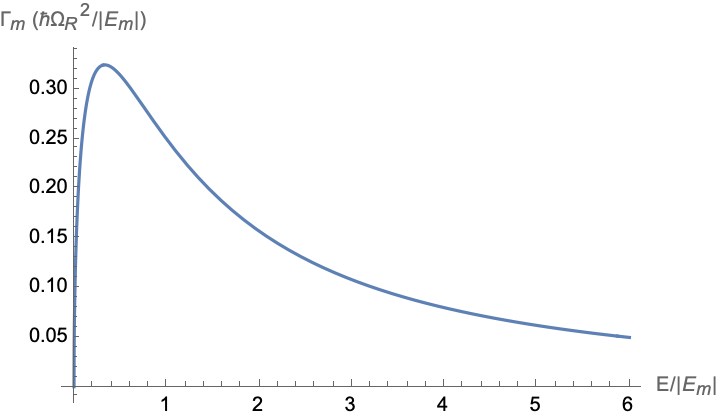
\includegraphics[width=0.7\textwidth]{gamma_m.png}
\end{figure}

When evaluated at $E = \hbar \omega + E_m$. $\Gamma_m(E)$ gives us the rf spectrum obtained from Fermi's golden rule, assuming weak and long drive. From the plot above, this is clearly not a Lorentzian. 

For $E$ near 0, we have
\begin{align*}
\Gamma_m(E) \approx \f{\hbar \Omega_R^2   E^{1/2}}{\abs{E_m}^{3/2}} + \dots 
\end{align*}
So, $\Gamma_m(E)$ goes like $E^{\be}$ with $\be = 1/2$ for $E$ near 0. 





% c
\item At large energies $E \gg \abs{E_m}$, we find that
\begin{align*}
\Gamma_m(E) \approx \f{\hbar \Omega_R^2\sqrt{\abs{E_m}}}{E^{3/2}} = \f{1}{a} \sqrt{\f{1}{2\mu}} \hbar^2 \Omega_R^2 \f{1}{E^{3/2}}
\end{align*}
By putting  
\begin{align*}
\Gamma_m(E) = \f{C}{8\pi} \sqrt{\f{1}{2\mu}} \hbar^2 \Omega_R^2 \f{1}{E^{3/2}},
\end{align*}
we find that
\begin{align*}
C = \f{8\pi }{a}.
\end{align*}
This is the \textit{contact} of a molecule. Let us also get $C$ from the relation given in the problem statement:
\begin{align*}
C = -\f{8\pi \mu}{\hbar^2} \f{\p E_m}{\p a^{-1}} = -\f{8\pi \mu}{\hbar^2} \f{\p}{\p a^{-1}} \lp -\f{\hbar^2}{2a^2 \mu} \rp = \f{8\pi}{a}. \quad\quad \checkmark
\end{align*}
So we're good. We see that the contact is related to the change in the molecular energy w.r.t $a$. \\

Finally, let us calculate the following integral:
\begin{align*}
\Omega_1^2 = \f{2}{\pi \hbar} \int_{-\infty}^\infty \Gamma_m(E) dE =  \f{2}{\pi \hbar} \int_{-\infty}^\infty \f{\hbar \Omega_R^2 \sqrt{E \abs{E_m}}}{(E + \abs{E_m})^2} dE = \Omega_R^2. 
\end{align*}
This could be done by hand, or in Mathematica:
\begin{lstlisting}
In[112]:= Integrate[(2/(Pi*h))*h*OR^2*Sqrt[e*EM]/(e + EM)^2, {e, 0, 
  Infinity}]

Out[112]= ConditionalExpression[OR^2, 
And[3 Arg[EM^(-1)] <= 2 Pi, Or[Re[EM] >= 0, And[NotElement[EM,Reals], 
Or[Im[EM] > 0, Im[EM] <= 3^Rational[1, 2] Re[EM]]]]]]
\end{lstlisting}

% d
\item Now we turn our attention to the energy shift. Let us calculate $\Delta_m(E)$ via $\Gamma_m(E)$ via the Kramer-Kronig's relation:
\begin{align*}
\Delta_m(E) 
&= \f{1}{2\pi}\mathcal{P} \int \f{\Gamma_m(E')}{ E - E'} \,dE' \\
&= \f{1}{2\pi}\mathcal{P} \int \f{\hbar \Omega_R^2 \sqrt{E' \abs{E_m}}}{ (E + \abs{E_m})^2(E - E')} \,dE' \\
&= 
\begin{cases}
\f{\hbar \Omega_R^2}{4 \abs{E_m}} \f{E/\abs{E_m} - 1}{(E/\abs{E_m} + 1 )^2} \quad\quad \text{ for } E > 0 \\ 
\f{\hbar \Omega_R^2}{4 \abs{E_m}} \f{ -1 }{\lp 1 + \sqrt{-E/\abs{E_m}} \rp^2} \quad\quad \text{ for } E \leq  0. 
\end{cases}
\end{align*}
For $\abs{E} \gg \abs{E_m}$, we have
\begin{align*}
\Delta_m(E) \approx \f{\hbar \Omega_R^2}{4\abs{E}}.
\end{align*}

%\begin{figure}[!htb]
%\begin{minipage}{0.45\textwidth}
%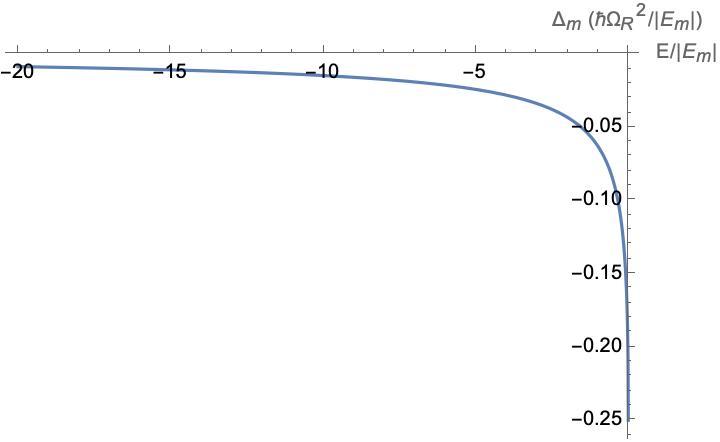
\includegraphics[width=0.98\textwidth]{delta_m_neg.png}
%\caption{$E\leq 0$}
%\end{minipage}
%\begin{minipage}{0.45\textwidth}
%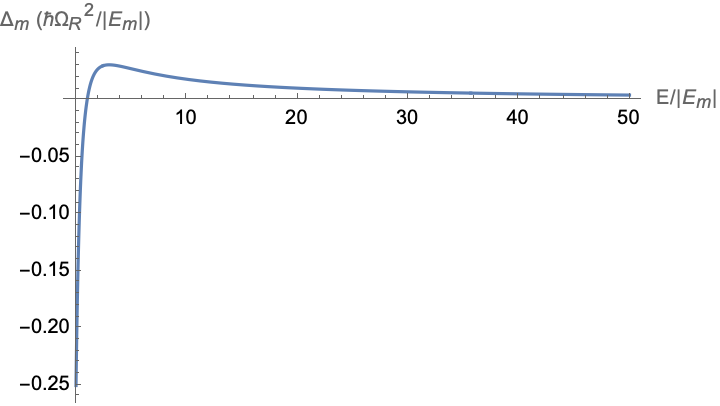
\includegraphics[width=0.98\textwidth]{delta_m.png}
%\caption{$E>0$}
%\end{minipage}
%\end{figure}

\begin{figure}[!htb]
\centering
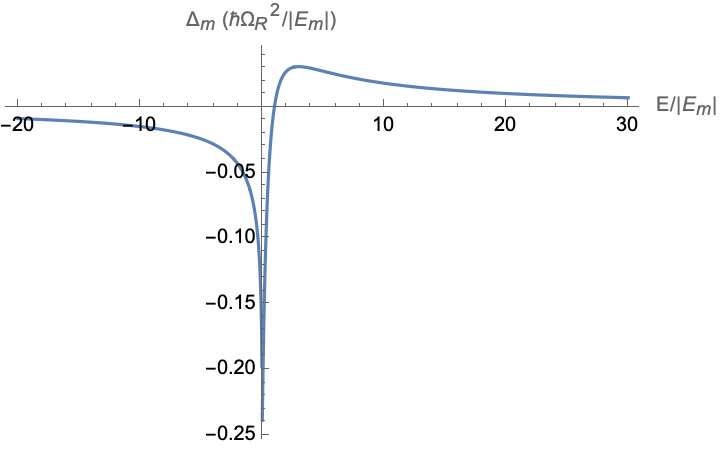
\includegraphics[width=0.6\textwidth]{delta_m_new.png}
\caption{Plot of $\Delta_m(E)$}
\end{figure}


% e
\item We now have all the ingredients to calculate the full time evolution:
\begin{align*}
U_m(\tau) = \int_{-\infty}^\infty \mathcal{U}_m(E) e^{-i E \tau/\hbar} \,dE
\end{align*}
where
\begin{align*}
\mathcal{U}_m(E) 
&= \f{1}{2\pi i} (G_{m-} (E) - G_{m+}(E)) \\
&= \lim_{\eta \to 0_+} \f{1}{\pi} \f{\hbar \Gamma_m(E) / 2 + \eta}{ [E - E_m - \hbar \omega - \hbar \Delta_m(E)]^2 + [\hbar \Gamma_m(E) /2 + \eta]^2} .
\end{align*}

Before doing any calculation, let's visualize $\mathcal{U}_m(E)$ first. We want to write $\mathcal{U}_m(E)$ entirely in terms of $x = E/\abs{E_m}, y = \delta/\abs{E_m} = \hbar \omega/\abs{E_m} - 1, z = \eta/\abs{E_m}, \xi = \hbar \Omega_R/\abs{E_m}$. Here, we are taking $\delta$ as having units of energy. We can rewrite $\mathcal{U}_m(E)$ in terms of these parameters to get
\begin{align*}
\mathcal{U}_m(E)
&= \f{1}{\pi} \f{1}{\abs{E_m}} 
\f{ \f{\xi^2}{2} \f{\sqrt{x}}{(x+1)^2} + z}
{\lb x - y - \f{\xi^2}{4} \f{(x-1)}{(x+1)^2} \rb^2 + \lb \f{\xi^2}{2} \f{\sqrt{x}}{(x+1)^2} + z \rb^2} \quad \quad E > 0
\end{align*}
\begin{align*}
\mathcal{U}_m(E) = \f{1}{\pi} \f{1}{\abs{E_m}} \f{z}{ \lb x - y - \f{\xi^2}{4} \f{-1}{\lp 1 + \sqrt{-x} \rp^2} \rb^2 +  z^2} \quad\quad E \leq 0
\end{align*}

We now pick $z = \eta/\abs{E_m} = 0.01$ and plot $\mathcal{U}_m(E,\delta) = \mathcal{U}_m(x,y)$ for $x,y \in [-10,20]$ for $\xi = 2,8,20$. 

\begin{figure}[!htb]
\centering
\begin{minipage}{0.3\textwidth}
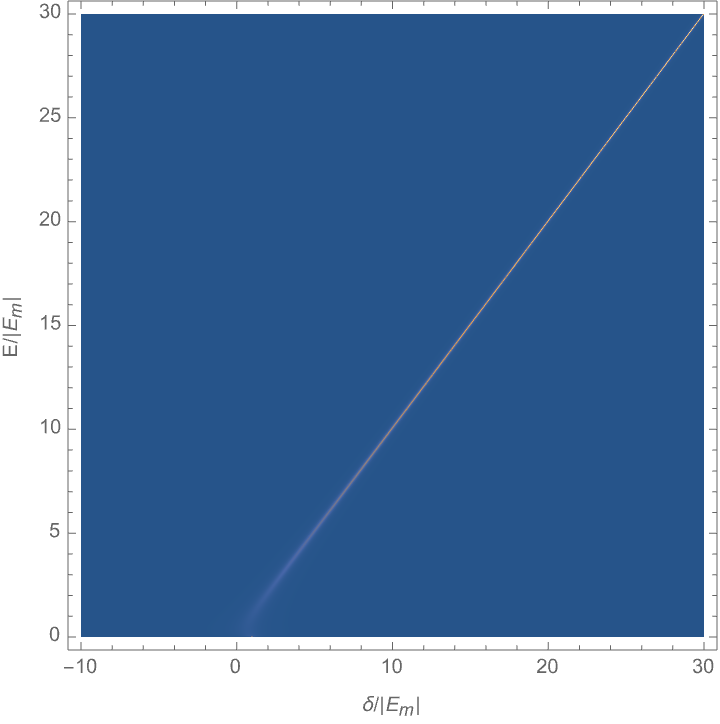
\includegraphics[width=0.9\textwidth]{UmE_density_plot.png}
\caption{$\xi = 2, E > 0$}
\end{minipage}
\begin{minipage}{0.3\textwidth}
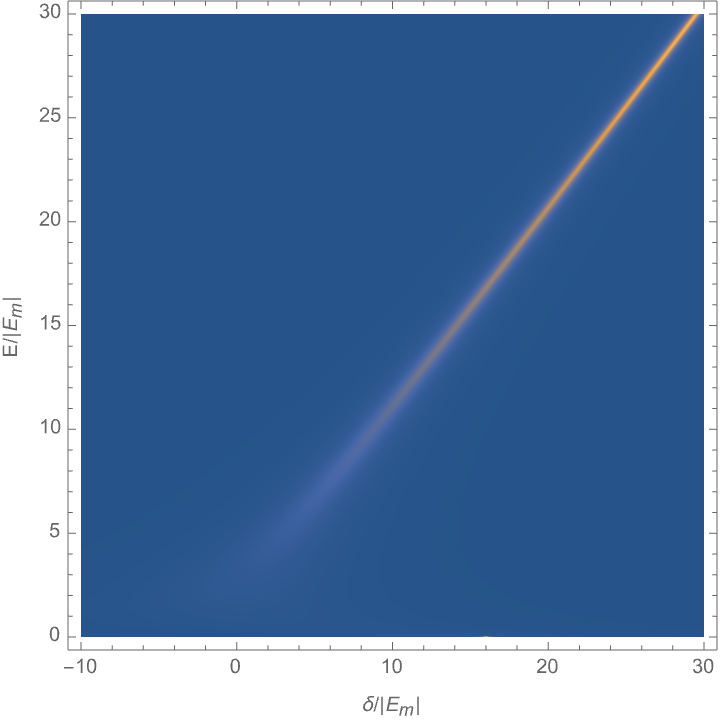
\includegraphics[width=0.9\textwidth]{UmE_density_plot_8.png}
\caption{$\xi = 8, E > 0$}
\end{minipage}
\begin{minipage}{0.3\textwidth}
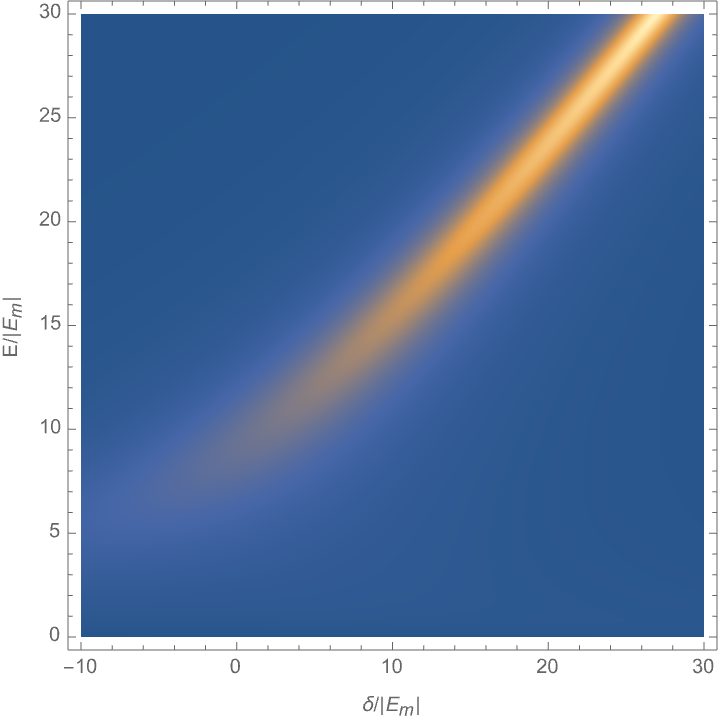
\includegraphics[width=0.9\textwidth]{UmE_density_plot_20.png}
\caption{$\xi = 20, E > 0 $}
\end{minipage}
\end{figure}

\begin{figure}[!htb]
\centering
\begin{minipage}{0.3\textwidth}
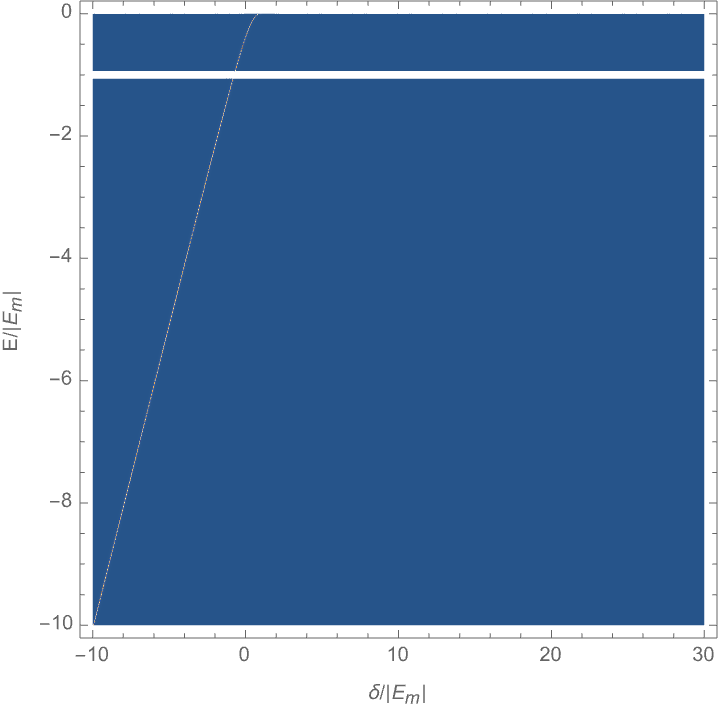
\includegraphics[width=0.9\textwidth]{UmE_density_plot_neg.png}
\caption{$\xi = 2, E \leq 0$}
\end{minipage}
\begin{minipage}{0.3\textwidth}
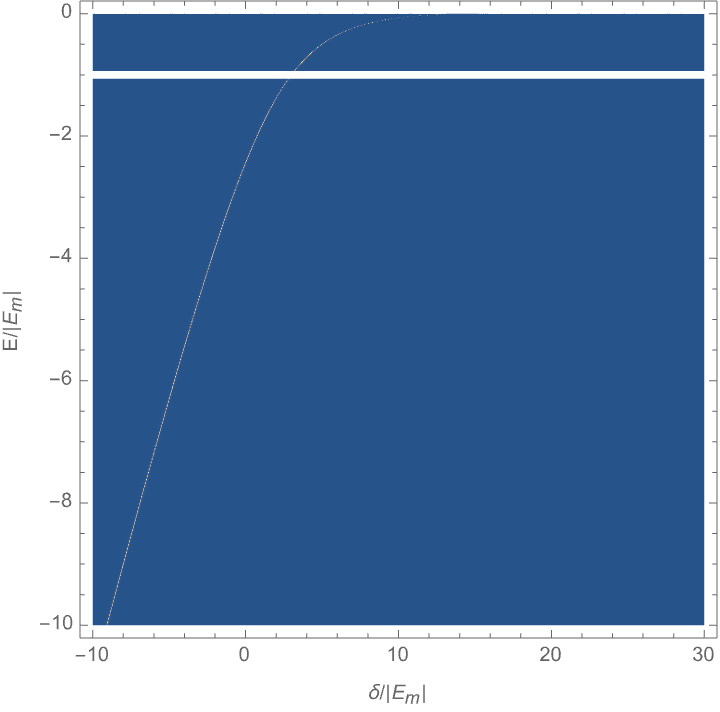
\includegraphics[width=0.9\textwidth]{UmE_density_plot_8_neg.png}
\caption{$\xi = 8, E \leq 0$}
\end{minipage}
\begin{minipage}{0.3\textwidth}
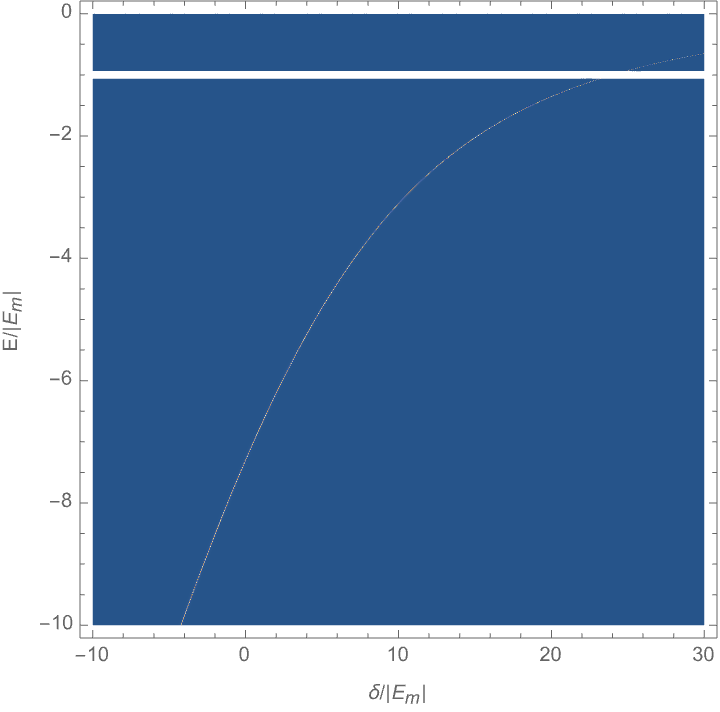
\includegraphics[width=0.9\textwidth]{UmE_density_plot_20_neg.png}
\caption{$\xi = 20, E \leq 0 $}
\end{minipage}
\end{figure}

\textcolor{purple}{The white horizontal line in the plots with $E\leq 0$ seems to be a glitch, but not really. Here, $\mathcal{U}_m(E)$ looks most like a $\delta$-function, and Mathematica can't properly scale its color.}

We are also asked to plot the normalized shift $4\Delta_m(E) \abs{E_m} / \hbar \Omega_R^2$ and the line $(E - \delta) \abs{E_m} / \hbar^2 \Omega_R^2$ as well as $\mathcal{U}_m(E)$ on the same graph. First, let us non-dimensionalize: 
\begin{align*}
\f{4\Delta_m(E) \abs{E_m}}{\hbar \Omega_R^2} 
&= \f{4}{\hbar \Omega_R^2} \f{\hbar \Omega_R^2}{4} \f{(E - \abs{E_m}) \abs{E_m} }{(E + \abs{E_m})^2} \ = \f{x - 1}{ (x+1)^2 } \text{ for } E  > 0 \\ 
&= \dots = \f{-1}{\lp 1 + \sqrt{-x} \rp^2} \text{ for } E \leq 0
\end{align*}
\begin{align*}
\f{(E - \delta)\abs{E_m}}{\hbar^2\Omega^2_R} = \f{x-y}{\xi^2}. 
\end{align*}


We are asked to pick $y = \delta / \abs{E_m} = 5$. The following plots show what happens for $\xi = \hbar \Omega_R / \abs{E_m} = 2, 10, 30$. 

\begin{figure}[!htb]
\centering
\begin{minipage}{0.32\textwidth}
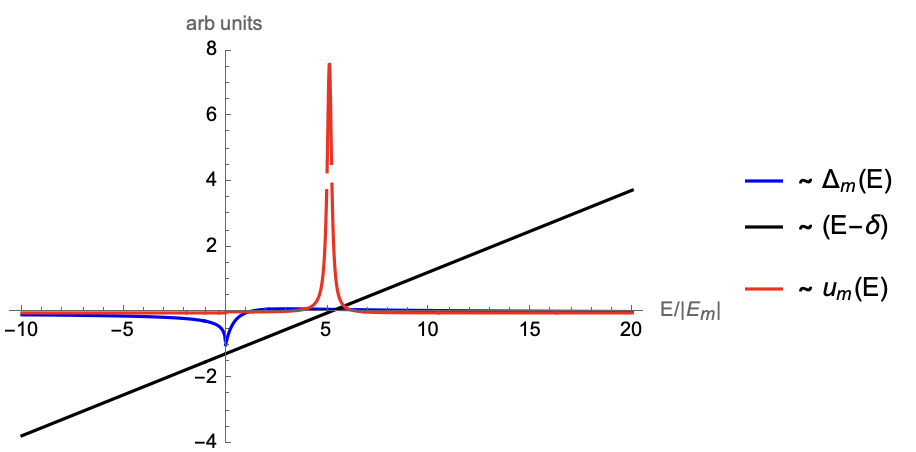
\includegraphics[width=0.98\textwidth]{new_2.png}
\caption{$\xi = 2$}
\end{minipage}
\begin{minipage}{0.32\textwidth}
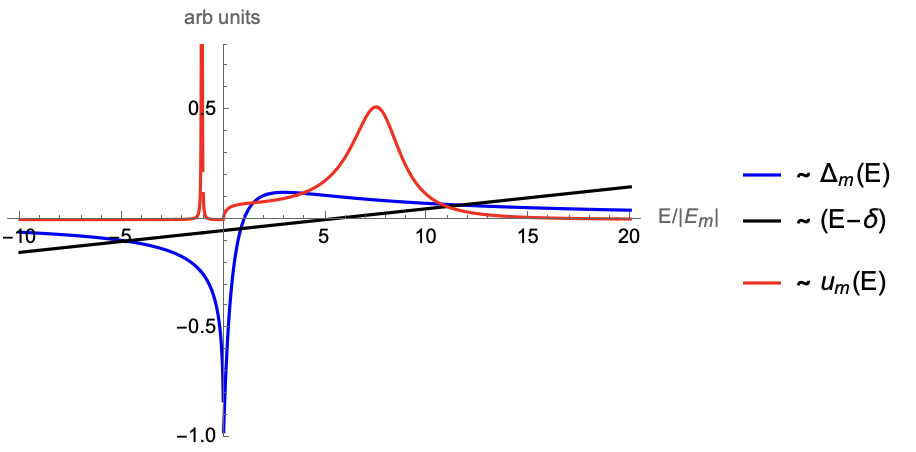
\includegraphics[width=0.98\textwidth]{new_10.png}
\caption{$\xi = 10$}
\end{minipage}
\begin{minipage}{0.32\textwidth}
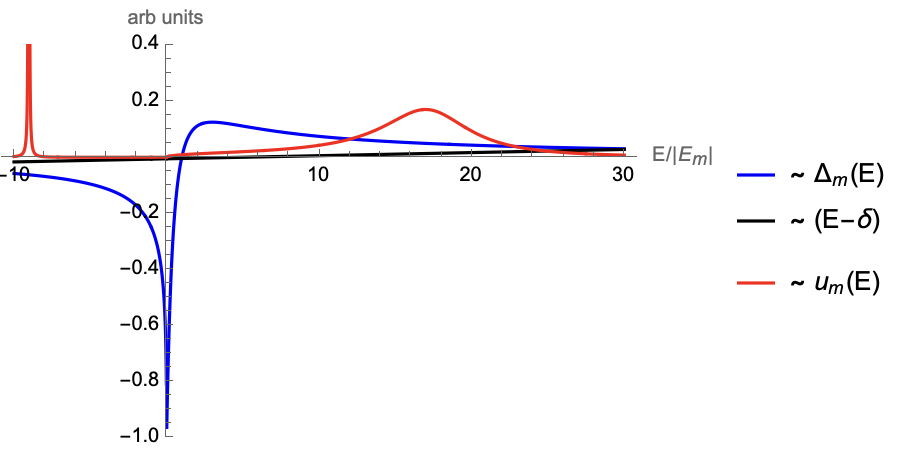
\includegraphics[width=0.98\textwidth]{new_30.png}
\caption{$\xi = 30$}
\end{minipage}
\end{figure}




% f
\item As we have seen from the previous part, for weak coupling $\mathcal{U}_m(E)$ is a $\delta$-function for $\delta < 0$, centered at $E = \hbar \delta$ (so $|U_m(\tau)|^2 = 1$) and approximately a Lorentzian of FWHM $\Gamma_m(\delta)$ for $E > 0$. The probability to stay in the state $\ket{m}$, $|U_m(\tau)|^2$ thus decays exponentially at rate $\Gamma_m(\hbar \delta)$. \\

However, at both short and long times, the exponential decay is not correct. First, at long times, the FT singles out only the portion of $U_m(E)$ for $E$ close to zero. Here, we want to deduce the dependence on $\tau$ of $U_m(\tau)$ at long times. To do this, we want to find the power law $\mathcal{U}_m(E) \propto E^\be$ for $E$ near zero. \\

We are interesting the regime where $x = E / \abs{E_m} >0$. Let $x\approx 0$. From the expression for $\mathcal{U}_m(E)$ for $E>0$, we can quickly find that $\mathcal{U}_m(E) \propto \sqrt{x}$ for $x\approx 0$. So the power law we get is $\mathcal{U}_m(E) \propto E^{1/2}$. With this, we have
\begin{align*}
U_m(\tau) \propto \int_0^{E_f = \hbar/\tau} E^{1/2} e^{-i E \tau / \hbar }\,dE \propto \lp \f{\hbar}{\tau} \rp^{3/2}.  
\end{align*}
Here, we have chosen the cutoff to be $E_f = \hbar / \tau$  due to dephasing of $e^{-i E \tau/\hbar}$. \\

In any case, we see that for long times, the decay follows a power law $\abs{U_m(\tau)}\propto 1/\tau^{3}$ as opposed to an exponential.



% g
\item Now we consider intermediate coupling strengths. As it turns out, for $\delta > 0$ there exists a critical coupling strength  $\Omega_{R,c}(\delta, \abs{E_m})$ for which a portion of the function $\mathcal{U}_m(E)$ acquires a $\delta$-function peak at $E < 0$. To find this critical coupling, let us look at $\mathcal{U}_m(E)$ for $E<0$ again:
\begin{align*}
\mathcal{U}_m(E) = \f{1}{\pi} \f{1}{\abs{E_m}} \f{z}{ \lb x - y - \f{\xi^2}{4} \f{-1}{\lp 1 + \sqrt{-x} \rp^2} \rb^2 +  z^2} \quad\quad E \leq 0
\end{align*}
In order to get a sharp peak in $\mathcal{U}_m(E)$ for $E<0$, we want the first term in the denominator to vanish:
\begin{align*}
x - y - \f{\xi^2}{4} \f{-1}{\lp1 + \sqrt{-x} \rp^2} = 0 \implies \xi^2 = 4(-x+y) \lp 1 + \sqrt{-x}\rp^2
\end{align*}
Reinstating dimensions, we get
\begin{align*}
\Omega_{R,c}^2 = \f{4}{\hbar^2}\abs{E_m}^2 \lp -\f{\abs{E}}{\abs{E_m}} + \f{\delta}{\abs{E_m}} \rp \lp 1 + \sqrt{\f{\abs{E}}{\abs{E_m}}} \rp^2\bigg\vert_{\abs{E} = ?}
\end{align*}
What should the value of $\abs{E}$ be here? The critical coupling is the minimum $\Omega_{R}$ for which the intersection between the $\Delta_m(E)$ and $(E-\delta)$ curves occur at $E<0$. In the expression above, $\Omega_{R,c}$ is decreasing as $E \to 0^-$. This means that we find $\Omega_{R,c}^2$ by simply setting $\abs{E} = 0$. The answer is therefore,
\begin{align*}
\Omega_{R,c}^2 = \f{4}{\hbar^2} \delta \abs{E_m}. 
\end{align*}
Following equation (29) of API, Section C$_\text{III}$.4, we can also calculate the critical coupling via:
\begin{align*}
\Omega_{R,c}^2 = \f{2\pi \delta}{\hbar \int_{-\infty}^\infty \, dE \, \Gamma'_m(E)/E} = \f{2\pi}{\hbar} \f{\delta}{ \hbar \pi / 2\abs{E_m}} = \f{4}{\hbar^2}\delta \abs{E_m}. \quad\quad\quad \checkmark
\end{align*}
Here, $\Gamma'_m(E)$ is the width normalized by the coupling $\Omega_R^2$: $\Gamma_m'(E) = \Gamma_m(E)/\Omega_R^2$. Also here we are treating $\delta$ as having units of energy. 

For larger coupling, we can find the energy of this discrete feature in terms of $\Omega_{R,c}^2, \Omega_{R}^2$, and $\abs{E_m}$ by first using the fact that 
\begin{align*}
\Delta_m(E) \approx \f{\hbar \Omega_R^2}{4E}. 
\end{align*}
The desired value for $E$ is the solution to the equation:
\begin{align*}
E - E_m - \hbar \omega - \hbar \Delta_m(E) = 0 \iff 
E = \delta + \f{\hbar^2 \Omega_R^2}{4{E}} = \f{\hbar^2 \Omega_{R,c}^2}{4\abs{E_m}} + \f{\hbar^2 \Omega_R^2}{4{E}}
\end{align*}
This is a quadratic equation and we're looking for negative solution $E<0$. Solving gives
\begin{align*}
E = \f{ \hbar^2 \Omega_{R,c}^2}{8 \abs{E_m}} - \f{1}{8\abs{E_m}}\sqrt{ 16\abs{E_m}^2 \hbar^2 \Omega_R^2 + \hbar^4 \Omega_{R,c}^4 }.
\end{align*}

% h
\item For strong coupling, $\Omega_R \gg \Omega_{R,c}$, there are two features in $\mathcal{U}_m(E)$ which both contribute to $U_m(\tau)$. The feature for $E<0$ is a $\delta$-function. The feature for $E>0$ is a broad Lorentzian-type feature. 

\begin{figure}[!htb]
\centering
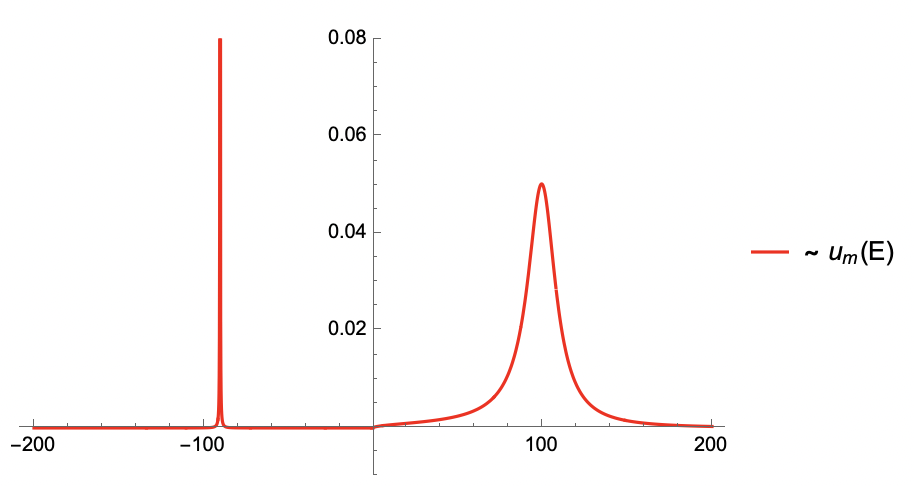
\includegraphics[width=0.7\textwidth]{two_peaks_newest.png}
\caption{Two features in $\mathcal{U}_m(E)$, for $\xi = \Omega_R / \abs{E_m} = 200$ and $\delta/\abs{E_m} = 0.5$. The features occur at $E \approx \pm 100$, which are roughly $\pm\xi/2$, as expected from the solution from Part (h) in the strong coupling limit $\Omega_R \gg \Omega_{R,c}$.}
\end{figure}

The locations of these peaks are found by finding the locations of the maxima of $\mathcal{U}_m(E)$. For $E<0$, we find from the previous part:
\begin{align*}
E_{<0} = \f{ \hbar^2 \Omega_{R,c}^2}{8 \abs{E_m}} - \f{1}{8\abs{E_m}}\sqrt{ 16\abs{E_m}^2 \hbar^2 \Omega_R^2 + \hbar^4 \Omega_{R,c}^4 } \approx - \f{\hbar \Omega_R}{2}.
\end{align*}
To find $E_{>0}$ exactly will be a bit cumbersome, so as an approximation we may use the positive solution to the quadratic equation in Part (h). In the strong coupling limit, we find that
\begin{align*}
E_{>0} \approx +\f{\hbar \Omega_R}{2}.
\end{align*}

How much weight is in either feature? Let's first "massage" the expression for $\mathcal{U}_m(E)$ so that it can be written in terms of $E_{<0}$ and as a $\delta$-function peak multiplied by some weight. Following Section 6. on page 251 on API, we can write, for $E\approx E_{<0}$, 
\begin{align*}
E - E_m - \hbar \omega - \hbar \Delta_m(E) 
&= \underbrace{E_{<0} - E_m - \hbar \omega - \hbar \Delta_m(E_{<0})}_{\approx 0} + E - E_{<0} - \hbar [\Delta_m(E) - \Delta_m(E_{<0})] \\
&= (E - E_{<0}) [ 1 - \hbar \Delta_m'(E_{<0}) ].
\end{align*}
With this, we find
\begin{align*}
\mathcal{U}_m(E) 
&= \lim_{\eta \to 0_+} \f{1}{\pi} \f{\hbar \Gamma_m(E) / 2 + \eta}{ [E - E_{m} - \hbar \omega - \hbar \Delta_m(E)]^2 + [\hbar \Gamma_m(E) /2 + \eta]^2} \\
&= \f{1}{1 - \hbar \Delta_m'(E_{<0})} \lim_{\eta \to 0_+} \f{1}{\pi} \f{\hbar \gamma_{<0}/2}{(E-E_{<0})^2 + (\hbar \gamma_{<0}/2)^2}
\end{align*}
where
\begin{align*}
\hbar \gamma_{<0} = \f{2\eta + \hbar \Gamma_m(E_{<0})}{1 - \hbar \Delta'_m(E_{<0})} = \f{2\eta}{1 - \hbar \Delta'_m(E_{<0})} 
\end{align*}
since $\Gamma_m(E) = 0$ for all $E < 0$. As $\eta \to 0^+$ and  $\Delta'_m(E_{<0}) \to 0$ as $E_{<0}$ remains finite, we see that the term with the limit turns into a $\delta$-function, and $\mathcal{U}_m(E)$ becomes a $\delta$-function multiplied by a weight which is the leading factor. Evaluating this factor is rather simple:
\begin{align*}
\Delta_m'(E_{<0}) = \f{\p}{\p {E}} \f{\hbar \Omega_R^2}{4E} \bigg\vert_{E = -\hbar \Omega_R/2} =  -\f{\hbar \Omega_R^2}{4\hbar^2 \Omega_R^2/4 } =  -\f{1}{\hbar}.
\end{align*}
Plugging this into the pre-factor, we get the weight of the $\delta$-function piece:
\begin{align*}
\f{1}{1 - \hbar \Delta'_m(E_{<0})} = \f{1}{1 - \hbar (-1/\hbar)} = \f{1}{2}.
\end{align*}

Now we find the weight of the Lorentzian piece. Near $E_{>0}$, the function $\mathcal{U}_m(E)$ is given as 
\begin{align*}
\mathcal{U}_m(E) 
&= \lim_{\eta \to 0_+} \f{1}{\pi} \f{\hbar \Gamma_m(E) / 2 + \eta}{ [E - E_{m} - \hbar \omega - \hbar \Delta_m(E)]^2 + [\hbar \Gamma_m(E) /2 + \eta]^2} \\
&= \f{1}{1 - \hbar \Delta_m'(E_{>0})} \lim_{\eta \to 0_+} \f{1}{\pi} \f{\hbar \gamma_{>0}/2}{(E-E_{>0})^2 + (\hbar \gamma_{>0}/2)^2}.
\end{align*}

However, this is no longer a $\delta$-function feature since $\Gamma_m(E) > 0$ for $E>0$. Rather, it is a Lorentzian of width $\propto \gamma_{>0}$. Similar to what we just did, the weight of this Lorentzian is the same pre-factor, except with terms with the subscript $_{<0}$.  Evaluating $\Delta_m'(E_{<0})$ gives us (still) $-1/\hbar$, so we find the weight:
\begin{align*}
\f{1}{1 - \hbar \Delta_m'(E_{>0})} = \f{1}{1 - \hbar (-1/\hbar)} = \f{1}{2},
\end{align*}
which is the same as the weight of the $\delta$-function feature. \\

Finally, we want to describe the evolution of the probability $\abs{U_m(\tau)}^2$ to stay in the molecular state for times short and long compared to the inverse width of the broad Lorenztian at $E>0$. To first order, we see that $U_m(\tau)$ is basically:
\begin{align*}
U_m(\tau) = \f{1}{2} e^{-i E_{<0} \tau / \hbar} + \f{1}{2} e^{-i E_{>0} \tau/\hbar} = \cos \lp \f{\hbar \Omega_R}{2} \tau \rp,
\end{align*}
so $\abs{U_m(E)}^2$ has Rabi oscillations at frequency $\hbar \Omega_R$. However, there are corrections in the long and short time regimes. In the short-time regime, i.e. for $\tau \ll 1 / \gamma_{>0}$, the contribution due to the Lorentzian feature is significant but is damped. The result is damped Rabi oscillations with time constant $1/\gamma_{>0}$. In the long-time regime, i.e. for $\tau \gg 1 / \gamma_{>0}$, there's only the contribution due to the $\delta$-function feature which has no damping. In this case, $\abs{U_m(\tau)} = \abs{e^{-i E_{<0} \tau / \hbar}}$ = 1. There is no more Rabi oscillation. \\

To see this more concretely let us make an example where the function $\mathcal{U}_m(E)$ is a equally-weighted sum of a $\delta$-function center at $E = -1$ and a Lorentzian centered at $E = 1$ with FWHM of $0.2$:
\begin{align*}
\mathcal{U}_m(E) = \delta(E+1) + \f{1}{2\pi} \f{0.2}{(E-1)^2 + (0.2)^2/4}.
\end{align*}

\begin{figure}[!htb]
\centering
\begin{minipage}{0.45\textwidth}
\centering
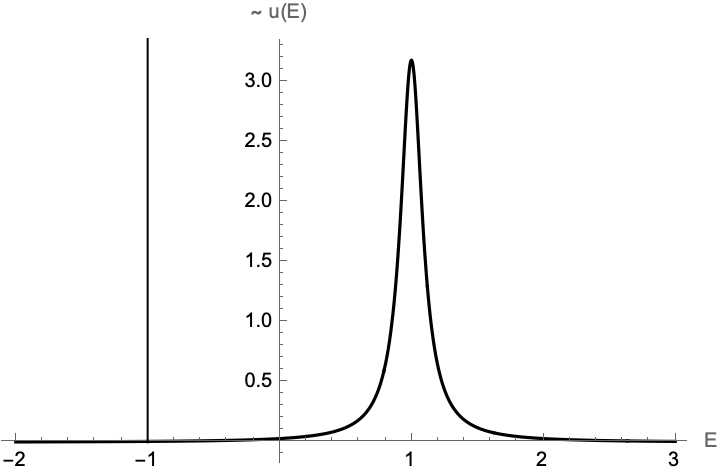
\includegraphics[width=0.92\textwidth]{dummy_UmE.png}
\caption{Dummy $\mathcal{U}_m(E)$.}
\end{minipage}
\begin{minipage}{0.45\textwidth}
\centering
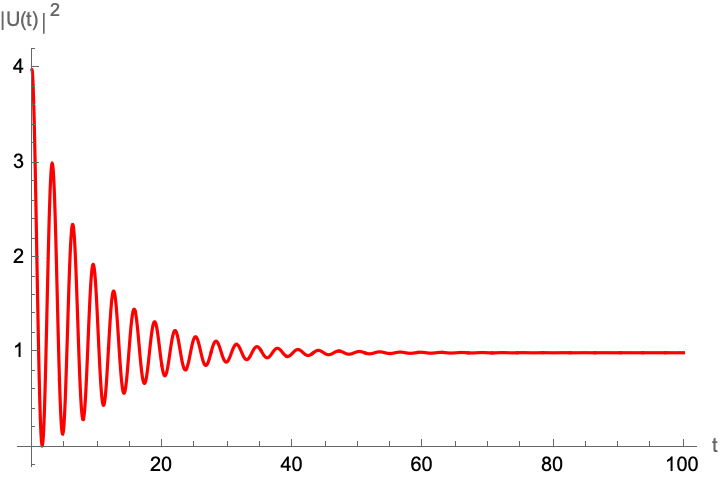
\includegraphics[width=0.92\textwidth]{dummy_UmT.png}
\caption{Dummy $\abs{{U}_m(\tau)}^2$.}
\end{minipage}
\end{figure}

We can numerically compute $\abs{U_m(\tau)}^2$ in Mathematica and plot it as a function of $\tau$. We observe damped Rabi oscillation. For short times, $\tau < 1/0.2 = 5$, we see damped Rabi oscillation. For long times $\tau \gg 5$, there are no more Rabi oscillations. 




\end{enumerate}




\end{document}








